%%% LaTeX Template: Designer's CV
%%%
%%% Source: http://www.howtotex.com/
%%% Feel free to distribute this template, but please keep the referal to HowToTeX.com.
%%% Date: March 2012


%%%%%%%%%%%%%%%%%%%%%%%%%%%%%%%%%%%%%
% Document properties and packages
%%%%%%%%%%%%%%%%%%%%%%%%%%%%%%%%%%%%%
\documentclass[a4paper,10pt,final]{memoir}


% misc
%\renewcommand{\familydefault}{bch}	% font
\usepackage{microtype}
\usepackage[]{fontspec}
%\setmainfont[Mapping=tex-text, Numbers={OldStyle, Proportional}]{Arno Pro}
% \setmainfont[Mapping=tex-text, Numbers={OldStyle,
%   Proportional}]{Frutiger LT Std 47 Light Condensed}
\setmainfont[Mapping=tex-text, Numbers={OldStyle, Proportional},
  Path = /Users/ras/Library/Fonts/ ,
  BoldFont = SeroPro-Bold.otf,
  ItalicFont = SeroPro-Italic.otf ,
  BoldItalicFont = SeroPro-BoldItalic.otf]{SeroPro.otf}
\newfontfamily\med[Mapping=tex-text, Numbers={OldStyle, Proportional},
%  Path = /Users/ras/Library/Fonts/]{SeroPro-ExtraLight.otf}
  Path = /Users/ras/Library/Fonts/]{SeroPro-Medium.otf}
\newfontfamily\light[Mapping=tex-text, Numbers={OldStyle, Proportional},
%  Path = /Users/ras/Library/Fonts/]{SeroPro-ExtraLight.otf}
  Path = /Users/ras/Library/Fonts/]{SeroPro-Light.otf}
\newfontfamily\lightit[Mapping=tex-text, Numbers={OldStyle, Proportional},
%  Path = /Users/ras/Library/Fonts/]{SeroPro-ExtraLight.otf}
  Path = /Users/ras/Library/Fonts/]{SeroPro-LightItalic.otf}
\newfontfamily\black[Mapping=tex-text, Numbers={Lining, Proportional},
  Path = /Users/ras/Library/Fonts/]{SeroPro-Black.otf}

% Letterspacing
\usepackage{soul}
\sodef\allcapsspacing{\upshape}{0.15em}{0.65em}{0.6em}%
\sodef\lowsmallcapsspacing{\scshape}{0.075em}{0.5em}{0.6em}%
\DeclareRobustCommand{\spacedallcaps}[1]{\MakeTextUppercase{\allcapsspacing{#1}}}%   
\DeclareRobustCommand{\spacedlowsmallcaps}[1]{\MakeTextLowercase{\textsc{\lowsmallcapsspacing{#1}}}}%

\pagestyle{empty}					% no pagenumbering
\setlength{\parindent}{0pt}			% no paragraph indentation


\DisemulatePackage{setspace}
\usepackage{setspace}
\setstretch{1.125} % Additional space between lines

% required packages (add your own)
\usepackage{flowfram}										% column layout
\usepackage[top=2cm,left=1cm,right=2cm,bottom=3cm]{geometry}% margins
\usepackage{graphicx}										% figures
\usepackage{url}											% URLs
\usepackage[usenames,dvipsnames]{xcolor}					% color
\usepackage{multicol}										% columns env.
	\setlength{\multicolsep}{0pt}
\usepackage{paralist}										% compact lists
\usepackage{tikz}
\definecolor{SpotColor}{rgb}{.445, .22, .216}

\usepackage{hyperref}
\hypersetup{%
    colorlinks=true, linktocpage=true, pdfstartpage=3, pdfstartview=FitV,%
    % uncomment the following line if you want to have black links (e.g., for printing)
    %colorlinks=false, linktocpage=false, pdfborder={0 0 0}, pdfstartpage=3, pdfstartview=FitV,% 
    breaklinks=true, pdfpagemode=UseNone, pageanchor=true, pdfpagemode=UseOutlines,%
    plainpages=false, bookmarksnumbered, bookmarksopen=true, bookmarksopenlevel=1,%
    hypertexnames=true, pdfhighlight=/O,%hyperfootnotes=true,%nesting=true,%frenchlinks,%
    urlcolor=SpotColor, linkcolor=SpotColor, citecolor=SpotColor, %pagecolor=SpotColor,%
    %urlcolor=Black, linkcolor=Black, citecolor=Black, %pagecolor=Black,%
    pdftitle={Resume},%the title
    pdfauthor={Rasmus Borgsmidt},%your name
    pdfsubject={},%
    pdfkeywords={},%
    pdfcreator={XeLaTeX},%
    pdfproducer={XeLaTeX}%
}

%%%%%%%%%%%%%%%%%%%%%%%%%%%%%%%%%%%%%
% Create column layout
%%%%%%%%%%%%%%%%%%%%%%%%%%%%%%%%%%%%%
% define length commands
\setlength{\vcolumnsep}{\baselineskip}
\setlength{\columnsep}{\vcolumnsep}

% left frame
\newflowframe{0.2\textwidth}{\textheight}{0pt}{0pt}[left]
\newlength{\LeftMainSep} \setlength{\LeftMainSep}{0.2\textwidth}
\addtolength{\LeftMainSep}{1\columnsep}   % small static frame for the vertical line
\newstaticframe{1.5pt}{\textheight}{\LeftMainSep}{0pt}
% content of the static frame
\begin{staticcontents}{1} \hfill \tikz{%
\draw[color=SpotColor,line width=1pt,yshift=0]
(0,0) -- (0,\textheight);}%
 \hfill\mbox{} \end{staticcontents}
%right frame
\addtolength{\LeftMainSep}{1.5pt}
\addtolength{\LeftMainSep}{1\columnsep}
\newflowframe{0.7\textwidth}{\textheight}{\LeftMainSep}{0pt}[main01] 


%%%%%%%%%%%%%%%%%%%%%%%%%%%%%%%%%%%%%
% define macros (for convience)
%%%%%%%%%%%%%%%%%%%%%%%%%%%%%%%%%%%%%
\newcommand{\Sep}{\vspace{1.5em}}
\newcommand{\SmallSep}{\vspace{0.5em}}
\newcommand{\MedSep}{\vspace{1em}}
\newcommand{\Dot}{\mbox{\color{SpotColor}$\,\;$\textbf{\char"00BB}$\,\;$}}
\newcommand{\NoSpaceDot}{\mbox{\color{SpotColor}\textbf{\char"00BB}}}

\newenvironment{inlinepar}[1]
	{\ignorespaces{\lowsmallcapsspacing{\textbf{#1}}}}
	{\ignorespacesafterend}

\newcommand{\CVSection}[1]
	{\textbf{\spacedallcaps{#1}}\par
	\SmallSep\normalsize\normalfont}

\newcommand{\CVSectionAnd}[2]
	{\textbf{\spacedallcaps{#1}\mbox{$\;\;$\lowsmallcapsspacing{and}$\;\;$}\spacedallcaps{#2}}\par
	\SmallSep\normalsize\normalfont}

\newcommand{\CVSectionCtd}[1]
	{\textbf{\spacedallcaps{#1}}$\;$ {\em (continued)}\par
	\SmallSep\normalsize\normalfont}

\newcommand{\CVItem}[1]
	{\textit{\color{SpotColor} #1}}

%%%%%%%%%%%%%%%%%%%%%%%%%%%%%%%%%%%%%
% Begin document
%%%%%%%%%%%%%%%%%%%%%%%%%%%%%%%%%%%%%
\begin{document}

% Left frame
%%%%%%%%%%%%%%%%%%%%
\begin{figure}
	\hfill
	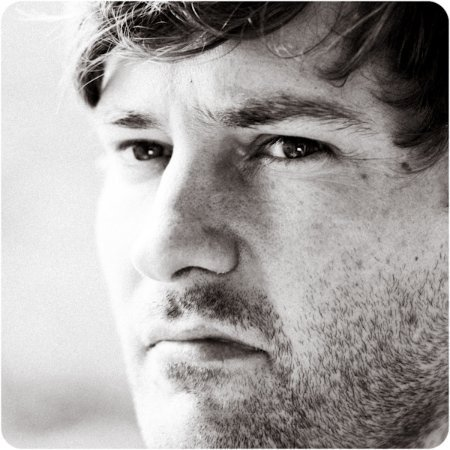
\includegraphics[width=0.6\columnwidth]{../media/borgsmidt.jpg}
	\vspace{-7cm}
\end{figure}

\begin{flushright}\footnotesize
  +45 70 71 03 23\\
  \href{mailto:rasmus@borgsmidt.dk}{rasmus@borgsmidt.dk}\\
  \href{http://dk.linkedin.com/in/borgsmidt}{linkedin.com/in/borgsmidt}\\
  \href{https://github.com/borgsmidt}{github.com/borgsmidt}\\[12pt]
  {\em References available\\ upon request}
\end{flushright}\normalsize
\framebreak

\fontdimen2\font=1.25\fontdimen2\font% interword space
\fontdimen3\font=1.25\fontdimen3\font% interword stretch
\fontdimen4\font=\fontdimen4\font% interword shrink

% Right frame
%%%%%%%%%%%%%%%%%%%%
\huge{\textbf{Rasmus Borgsmidt}} \\
\Large{\color{SpotColor}\em Sr Software Engineer,$\;$ B.Sc.~in Computer Science}

\normalsize\normalfont

\Sep\begin{inlinepar}{about me}
  Born 1975 and grew up in the Copenhagen area\Dot Tinkering with computers
  since the 1980s\Dot Bachelor of Computer Science from University of
  Copenhagen\Dot Hired into Adaytum in 1997, then acquired by \mbox{Cognos} in
  2003 and IBM in 2009\Dot 15+ years of experience building financial planning
  software for the enterprise\Dot Worked on numerous projects and technologies,
  ranging from bare-metal machine coding to high-level object-oriented,
  functional and array languages\Dot Named inventor and co-inventor on several
  \mbox{issued} patents\Dot Lived abroad a number of years in the UK and
  Luxembourg\Dot Married, father of three, currently based in Copenhagen
\end{inlinepar}

\Sep\CVSection{work experience}

\CVItem{Sr Software Engineer,$\;$ IBM,$\;$ 2009--present}

In this role, my primary responsibility is refining and maintaining the calc
engine at the heart of the {\em IBM Cognos Planning} enterprise software
solution. I also contribute to the development of other related products and
occasionally visit customer sites for beta testing and the like.

\SmallSep\CVItem{Scrum Master for Distributed Team,$\;$ IBM,$\;$ 2009--2012}

In addition to my development responsibilities, I served as {\em Team Captain}
of a highly distributed scrum team with members across four time zones.

\SmallSep\CVItem{Sr Software Engineer,$\;$ Cognos,$\;$ 2003--2008}

In this role, my primary responsibility was building and maintaining core server
components of the {\em Cognos Planning} enterprise software solution. In
addition to this, I was heavily involved in research projects that later
resulted in a series of patents.

\SmallSep\CVItem{QA Technician / Software Engineer,$\;$ Adaytum,$\;$ 1997--2002}

In my initial role at Adaytum, I worked in 3rd-level support and with test bed
development. Later my responsibilities shifted and I started contributing
directly to the {\em Adaytum Planning} software product.

\Sep\CVSection{education}

\CVItem{B.Sc.~in Computer Science,$\;$ University of Copenhagen,$\;$ 2010--2014}

A bachelor's thesis was submitted June 2013 and was graded 12 (top mark). The
thesis titled {\em Functional Array Programming Compiled to a Virtual Machine}
is available upon request.

\SmallSep\CVItem{B.Sc.~in Computer Science,$\;$ Maths,$\;$ University of
  Copenhagen,$\;$ 1994--1998}

First attempt at this degree was cut short after being hired into Adaytum in
1997.

\Sep\CVSection{skills}

\begin{inlinepar}{programming}
  Experience with a host of languages, such as Java, Ruby, C\#, JavaScript,
  Haskell, SML, Erlang, C, Python, J/APL, MSIL, Java Bytecode, assembly
  language, \mbox{binary} machine code---the list goes on.
\end{inlinepar}

\SmallSep\begin{inlinepar}{methodology}
  Keen proponent of {\em outside-in} design principles, such as test-driven
  development, and the importance of small teams, incremental delivery and
  iterative processes in general. Respects the art and craft of software
  engineering, and takes pride in continuous integration and refactoring.
\end{inlinepar}\enlargethispage{2\baselineskip}\\

{\hfill\footnotesize\em continued overleaf}
\clearpage
\framebreak
\framebreak

\begin{inlinepar}{languages}
  Speaks and writes Danish and English with native proficiency, German with
  elementary proficiency.
\end{inlinepar}

\Sep\CVSection{personality}
\begin{inlinepar}{traits}
  Always curious, generally well-liked, can have a meaningful conversation with
  people from all walks of life. Handles pressure well and makes a point of
  doing things the right way.
\end{inlinepar}

\SmallSep\begin{minipage}{0.7\textwidth}
\begin{multicols}{3}
\begin{compactitem}[\hspace{12pt}\color{SpotColor}\NoSpaceDot]
	\item {\em team player}
        \item {\em thorough}
        \item {\em creative}
        \item {\em analytic}
        \item {\em leads by example}
        \item {\em professional}
\end{compactitem}
\end{multicols}
\end{minipage}\\

\SmallSep\begin{inlinepar}{interests}
  Concurrent Programming (Erlang/OTP)\Dot Dynamic and functional languages\Dot
  Building grammars and DSLs\Dot Cloud technologies\Dot Network security and
  anonymity\Dot Tinkering with Raspberry Pi\Dot Photography\Dot Classic computer
  emulation\Dot Go (ancient strategic board game)
\end{inlinepar}

\Sep\CVSection{patents}

\CVItem{Scalable mechanism for resolving cell-level access from sets of
  dimensional access rules},$\;$ 2013,$\;$ uspatno.~8,538,990\\[3pt]
Techniques for resolving cell-level access in a multi-dimensional data structure
based on one or more sets of dimensional access rules.\\[3pt]
Rasmus Borgsmidt, David Bowen, Kirk Bates

\MedSep\CVItem{Automatically moving annotations associated with
  multi-dimensional data be-\linebreak tween live data cubes},$\;$ 2013,$\;$
uspatno.~8,347,207\\[3pt]
Techniques for sharing multi-dimensional data and associated annotations between
software systems.\\[3pt]
Rasmus Borgsmidt, Finuala Barnes, Bindhu Cherian

\MedSep\CVItem{Enterprise planning and performance management system
  providing type-safe retrieval of multi-dimensional data},$\;$ 2011,$\;$
uspatno.~7,895,150\\[3pt]
Techniques for ensuring type safety at compile time of multi-dimensional data
retrieval.\\[3pt]
Rasmus Borgsmidt, Michael Gould

\MedSep\CVItem{Job scheduling for automatic movement of
  multi-dimensional data between live data cubes},$\;$ 2011,$\;$
uspatno.~7,877,355\\[3pt]
Techniques for sharing multi-dimensional data between software systems.\\[3pt]
Rasmus Borgsmidt, David Bowen

\MedSep\CVItem{Virtual multi-dimensional datasets for enterprise
  software systems},$\;$ 2010,\\
uspatno.~7,747,562\\[3pt]
Techniques for specifying virtual datasets within an enterprise
software system.\\[3pt]
Rasmus Borgsmidt, Michael Gould

\MedSep\CVItem{Multi-dimensional data cube validation},$\;$ 2009,$\;$
uspatno.~7,610,294\\[3pt]
Techniques for validating data that a user enters into a multi-dimensional data
cube within an enterprise software system.\\[3pt]
Rasmus Borgsmidt
\end{document}
